We now describe the overview of the \name{} protocol that localizes faults even on unreliable transmission channels, e.g., in the presence of interference from adversaries. %achieve robust and lightweight fault localization for source authenticity and path compliance. Fig. \ref{workflow} depicts the work flow of RLFL protocol, which contains three phases with different purposes, as described blow.
%\subsection{High-Level Steps}
%\label{highlevelsteps}
Note that, in \name{}, end-to-end communication sessions are divided into consecutive \emph{epochs} that vary with different sessions and their phases of the sessions. In one session, after {\tt S} sends a number of packets to {\tt D} or a period of time interval expires, the \emph{epoch} value will be updated. \name{} performs the verification during each epoch. 

Fig. \ref{workflow} shows the workflow of \name{} protocol. At the beginning, \name{} enables the source {\tt S} to establish symmetric keys with all the other entities on $\Psi$.  
Using the symmetric keys, the packets verification and fault localization will then be carried out. Concretely, before each packet's departure, {\tt S} firstly inserts and initializes \name{} packets. Each entity will verify and probabilistically sample the packets on receiving them. At the end of each epoch, {\tt S} will perform fault localization according to the sampling information of entities.
\begin{figure}%[H]
\begin{center}
  % Requires \usepackage{graphicx}
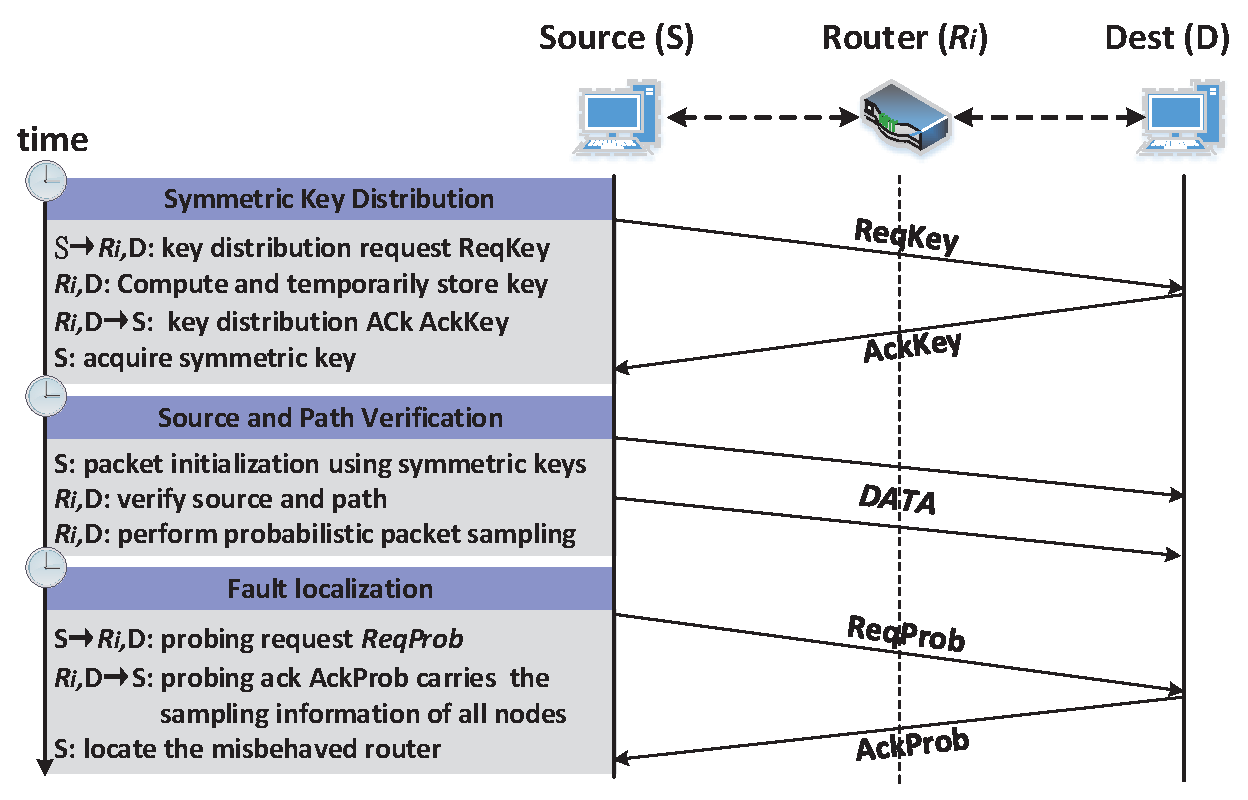
\includegraphics[width=8cm]{visio/workflow7.eps}
\caption{The workflow of \name{} protocol for the source ({\tt S}), intermediate entities (\emph{R}$_\emph{i}$) and the destination ({\tt D}), where ReqKey and AckKey (ReqProb and AckProb) respectively denote the request and acknowledgment messages for secret key distribution (fault localization) probing.}\label{workflow}
\end{center}
\vspace{-3mm}
\end{figure}\\
%RFL allows these entities to sign and verify packet information by using the keys such that it localizes faults.\\
%\noindent{\textbf{Symmetric key distribution.}} We propose a lightweight and anti-attack symmetric key distribution protocol called \emph{LASKey} to guarantee secure key distribution. As shown in Fig. \ref{workflow}, \emph{S} sends a request packet (denoted by ReqKey) along \emph{Path}$^\emph{*}$ towards \emph{D}. Each entity computes and temporarily store the symmetric key. Upon receiving the message, \emph{D} initializes and sends an ack packet (denoted by AckKey) back to \emph{S}, which would carry the encrypted symmetric key of each hop in the path and the signatures of these entities on reversed \emph{Path}$^\emph{*}$.
%Concretely, \emph{D} initializes and adds its encrypted \emph{K}$_{\emph{S,D}}$ to \emph{AckKey} packet; each router \emph{R}$_\emph{i}$ inserts its encrypted \emph{R}$_{\emph{S,R}_\emph{i}}$ and signatures into \emph{AckKey} packet before $\mathcal{T}_\emph{i}$ expires.
%Based on the received AckKey packet, \emph{S} decrypts and obtains the symmetric keys.\\
\noindent{\textbf{Robust symmetric key distribution.}}
\name{} introduce a robust symmetric key distribution called \namekey{} to guarantee secure key establishment and allocation between {\tt S} and network entities in forwarding path. As shown in Fig. \ref{workflow}, {\tt S} sends a request packet (denoted by ReqKey) along $\Psi$ towards {\tt D}. Each entity computes and temporarily store the symmetric key. Upon receiving ReqKey, {\tt D} initializes and sends an ack packet (denoted by AckKey) back to {\tt S}, which will gradually record the encrypted symmetric keys and signatures of each entity on $\Psi$ hop by hop during AckKey's delivery to {\tt S}.
Based on the received AckKey, {\tt S} decrypts and obtains the symmetric keys.\\
\noindent{\textbf{Lightweight source and path verification.}}
After obtaining the symmetric keys, {\tt S} precomputes a marking for each entity on $\Psi$ before sending out a data packet. All markings are inserted into a new header called \name{} header between IP header and TCP header.
During the packet transmission, each entity \emph{R}$_\emph{i}$ performs packet forwarding verification by recalculating its own marking using symmetric key \emph{K}$_{\emph{S,R}_\emph{i}}$ once receiving packets, and comparing it with the inserted one on \name{} header. Only these two values are equal, can \emph{R}$_\emph{i}$ forward the packet to downstream entities. Note that each intermediate entity \emph{R}$_\emph{i}$ does not require to store symmetric keys for each flow, which introduces the lightweight \name{} router.\\
%Note that the source address and the destination address is used as the input to compute each node's marking, which could defense source spoofing and traffic redirection. The address of one-hop upstream router as one input of marking computation prevent the forwarding path from deviation. Besides, marking calculation also employs TTL value and all downstream routers' markings to defense against frame attacks, such as TTL attack.
\noindent{\textbf{Robust fault localization.}}
\name{} enables entities to sample packets for fault localization. {\tt S} uses the packet sampling information of each entity on $\Psi$ to localize the fault. Our developed probabilistic packet sampling function $\mathcal{F}$ (described in Section \ref{faultlocalization}) determines which entity will sample the packet in one epoch. Each entity's packet sampling results can be only predicted by {\tt S}, but unknowable to others. Concretely, {\tt S} uses $\mathcal{F}$ to learn which entities will sample a packet. Upon receiving the packet, the entities (\emph{R}$_\emph{i}$ and {\tt D}) perform $\mathcal{F}$ to sample the packet and store the results in a bloom filter. At the end of each epoch, {\tt S} sends a request probing packet, called ReqProb, to ask all entities on $\Psi$ for their sampling information of this epoch. The ack message (denoted by AckProb) carrying the encrypted sampling information will be delivered from {\tt D} to {\tt S}.
Thereby, based on the received AckProb, {\tt S} determines where a fault occurs (detailed in Section \ref{faultlocalization}).\\
\indent
However, %\textcolor{red}{since the unreliable communication channels can tolerate corrupting fault localization,} 
it is challenging to implement \name{} because of the following issues:\\
\noindent \textbf{Corrupting symmetric key distribution.} The symmetric key is the important guarantee to correctly perform packet forwarding verification and fault localization. If the adversary maliciously corrupts symmetric key distribution (e.g., modify, drop and redirect the ReqKey or AckKey). \name{} will become paralyzed and unable to localize the fault. Meanwhile, if each entity needs to store one symmetric key per-session, the state exhaustion (e.g., DoS)  attacks will be easier to happen, which is infeasible in the practical networks.\\
\noindent{\textbf{Unreliable packet transmission.}} The adversary can destroy the transmission of request or ack packet for corrupting \name{}. When {\tt S} sends request packets (ReqKey and ReqProb), the misbehaved entity can drop or redirect these packets to disturb symmetric key distribution or {\tt S}'s obtaining sampling information. Thereby, any entity can not reply its symmetric key or packet sampling result back to {\tt S}, incurring the failure of fault localization. Also, the entity can modify the data of ack packets (AckKey and AckProb). Even though {\tt S} can capture the modified data by checking signatures on these ack packets, it can not identify and localize the fault.\\
\noindent{\textbf{Interference by frame attacks.}} The misbehaved entity can launch frame attacks to corrupt \name{}. This can try to make benign entities mistakenly perform packet forwarding verification, which can frame them for destroying reliable packet delivery. For example, TTL attack can be used to significantly decrease TTL value of any packets so as to frame the benign entity of dropping packets. Moreover, when performing source and path verification, the misbehaved entity can tamper the pre-inserted markings in \name{} header, resulting in the verification failure or packets discard to disturb the fault localization.
%In \name{} protocol, \emph{S} uses the packet sampling information of each node on \emph{Path}$^\emph{*}$ to determine the location of the fault. Our proposed probabilistic packet sampling function $\mathcal{F}$ (described in Section \ref{faultlocalization}) determines whether the current packet would be sampled at \emph{R}$_\emph{i}$ or \emph{D}. Each node's packet sampling results can be predictable by \emph{S}, but unknowable to other nodes.
%Before each packet's departure, \emph{S} uses $\mathcal{F}$ to learn which node(s) would sample this packet. When receiving the packet, \emph{R}$_\emph{i}$ and \emph{D} perform $\mathcal{F}$ to sample the packet and store it in a bloom filter. At the end of each epoch, \emph{S} send a request probing packet, called \emph{ReqProb}, to ask all nodes on \emph{Path}$^\emph{*}$ for their sampling information of this epoch. Then the ack probing packet called \emph{AckProb} is forwarded from \emph{D} to \emph{S}. When AckProb packet reaches each hop on \emph{Path}$^\emph{*}$, each node would add its own encrypted sampling information to AckProb. %Note that \emph{R}$_\emph{i}$ would send its own sampling information \emph{AckProb}$_\emph{i}$ back to \emph{S} when $\mathcal{T}_\emph{i}$ expires, as Section \ref{askeymechanismovervies} describes.
%Based on the received AckProb, \emph{S} determines the fault location according to the difference between the received sampling information and the predicted one of each node.
%We lower the storage overhead of each node by reducing the bloom filter length in the following ways: (i) the session is divided into consecutive epoches, enabling each node not have to sample all packets of the session; (ii) $\mathcal{F}$ provides probabilistic packet sampling, enabling each node not have to sample all packets of each epoch. Considering the transmission delay, two bloom filters for each node on \emph{Path}$^\emph{*}$ should be established and stored by \emph{S}, one for the current epoch and another for the next epoch. Meanwhile, each node also builds two bloom filters for the current and the next epoch. If the sampling information of one epoch is reported to \emph{S} and employed, the corresponding bloom filter would be emptied for the continuous usage.
%\subsection{Challenges in \name{} protocol}
%\label{challengesoverview}
%Based on the high-level description, \name{} protocol faces serious security vulnerabilities, especially in unreliable transmission channel, which allows the misbehaving router to disturb any form of fault localization.\\
%\noindent{\textbf{Disturbing the transmission of request and ack packet.}} When \emph{S} sends request packet ReqKey and ReqProb, the misbehaving router could drop or redirect these packet to disturb symmetric key distribution or fault localization. Unreceiving request packets, entities would not send their encrypted symmetric key or packet sampling information back to \emph{S}, causing the failure of fault localization. In addition to dropping or redirecting, the offending router could also modify the packet data of AckKey and AckProb. Even though knowing the packet data has already been maliciously modified checking signatures, \emph{S} could not identify and localize the fault.\\
%\noindent{\textbf{Launching the frame attacks to blame others.}} To evade to be localized, the misbehaving router could launch TTL attack by greatly decreasing TTL value of any received packets for framing other entities. Besides, when performing source and path verification, the misbehaving entity could modify the pre-inserted markings in \name{} header, causing the failure of verification, and packet dropping by other router, which disturbs the fault localization accuracy.

%\subsection{Lightweight and Anti-attack Key Distribution}
%\label{askeymechanismovervies}
%At the beginning of RLFL protocol, symmetric keys shared between \emph{S} and each node on \emph{Path}$^\emph{*}$ is established and distributed. We propose a lightweight and anti-attack symmetric key distribution mechanism, called \emph{LASKey}, to guarantee the security of key distribution. LASKey mechanism provides two vital properties. (i) Lightweight: each router do not have to store the symmetric key, regardless of the number of flows and sources. (ii) Anti-attack: \emph{S} could locate the misbehaved router who disturbs or destroys LASKey mechanism, which offers the robustness for symmetric key distribution.

%Consider the scenario of Fig. \ref{attackmodel}.
%When establishing symmetric keys, \emph{S} firstly sends request packet (denoted by \emph{ReqKey}) along \emph{Path}$^\emph{*}$ towards \emph{D}. Each router \emph{R}$_\emph{i}$ computes \emph{K}$_{\emph{S,R}_\emph{i}}$ and start the timer $\mathcal{T}_\emph{i}$ on receiving \emph{ReqKey} packet. When \emph{ReqKey} packet arrives at \emph{D}, the acknowledgment packet (denoted by \emph{AckKey}) is forwarded towards \emph{S}, which carries the encrypted symmetric keys and signatures of all nodes on reversed \emph{Path}$^\emph{*}$. Concretely, \emph{D} initializes and adds its encrypted \emph{K}$_{\emph{S,D}}$ to \emph{AckKey} packet; each router \emph{R}$_\emph{i}$ inserts its encrypted \emph{R}$_{\emph{S,R}_\emph{i}}$ and signatures into \emph{AckKey} packet before $\mathcal{T}_\emph{i}$ expires. Based on the received \emph{AckKey} packet, \emph{S} performs decryptions and obtains the symmetric keys.

%Note that all nodes on \emph{Path}$^\emph{*}$ would check the authenticity of \emph{ReqKey} and \emph{AckKey} packets by verifying the signatures when receiving these two packets. Due that the misbehaved router might modify, drop and redirect \emph{ReqKey} or \emph{AckKey} packet, \emph{R}$_\emph{i}$ might not receive \emph{AckKey} within timer threshold. In this case, \emph{R}$_\emph{i}$ initializes and sends \emph{AckKey}$_\emph{i}$ towards \emph{S}. \emph{R}$_{\emph{i-}1}$, $\cdots$, \emph{R}$_\emph{1}$ add their encrypted symmetric keys and signatures to \emph{AckKey}$_\emph{i}$. In this case, \emph{S} decrypts \emph{AckKey}$_\emph{i}$ instead of \emph{AckKey} packet, only obtaining \emph{K}$_{\emph{S,R}_1}$, $\cdots$, \emph{K}$_{\emph{S,R}_\emph{i}}$. This help to locate $\langle$\emph{R}$_\emph{i}$\emph{,R}$_{\emph{i+}1}$$\rangle$ as the fault.

%\subsection{Source and Path Verification}
%In order to achieve the source and path validation at each hop and prevent the destination from exhaustion, \emph{S} precomputes the marking for each node on \emph{Path}$^\emph{*}$ using the obtained symmetric key. These markings are all inserted into RLFL header, which is added between IP header and TCP/UDP header of IP packet. Once receiving the packet, \emph{R}$_\emph{i}$ recalculates its marking using \emph{K}$_{\emph{S,R}_\emph{i}}$ and compares it with the one on RLFL header. Only these two values is consistent, can \emph{R}$_\emph{i}$ forward the packet to downstream routers.

%Note that the source address and the destination address is used as the input to compute each node's marking, which could defense source spoofing and traffic redirection. The address of one-hop upstream router as one input of marking computation prevent the forwarding path from deviation. Besides, marking calculation also employs TTL value and all downstream routers' markings to defense against frame attacks, such as TTL attack. 